\documentclass[tikz,border=7mm]{standalone}
\usetikzlibrary{calc}
\begin{document}
  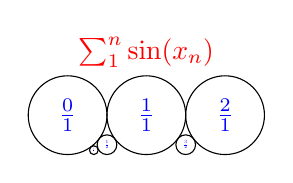
\begin{tikzpicture}
    \node[red] at (1,1.3) {$\sum_1^n \sin(x_n)$};
    \foreach[evaluate={\f=\p/\q;\r=1/(2*\q^2)}]
      \p/\q in {0/1,1/1,1/2,2/1,3/2,1/3}{
        \draw (\f,\r) circle(\r) node[blue,scale=2*\r]{$\frac{\p}{\q}$};
      }
  \end{tikzpicture}
\end{document}
